% ROLOpt.jl proof-of-concept evidence deck.
% Build:  make           (regenerates data, runs lualatex twice)
%   or:    /Library/TeX/texbin/lualatex slides.tex   (twice; data must exist)
% Data/tables under data/ and tables/ are produced by generate_evidence.jl.
\documentclass[aspectratio=169,10pt]{beamer}
\usetheme{default}
\setbeamertemplate{navigation symbols}{}
\setbeamertemplate{footline}[frame number]
\usepackage{booktabs}
\usepackage{siunitx}
\sisetup{output-exponent-marker=\text{e}}
\usepackage{pgfplots}
\pgfplotsset{compat=1.18}
\usepgfplotslibrary{groupplots}
\usetikzlibrary{positioning,arrows.meta}

\setbeamercolor{frametitle}{fg=blue!55!black}
\setbeamerfont{frametitle}{size=\normalsize,series=\bfseries}

\newcommand{\fdata}[1]{data/#1}

\begin{document}

% ---------------------------------------------------------------- Frame 1
\begin{frame}{ROLOpt.jl: an inexact proximal trust region for risk-averse optimization}
  \small
  Solves \;$\displaystyle \min_x\; J(x)=f(x)+\sigma_A\!\big(F(x)\big)+\varphi(x)$
  \hfill{\tiny Kouri, arXiv:2604.07216v1 \;$\cdot$\; ports Trilinos ROL \texttt{TypeP} @\,\texttt{46b83e0}}

  \smallskip
  {\footnotesize $f$ smooth, $F:X\!\to\!Y$ smooth, $\varphi$ prox-friendly, $\sigma_A$ the support function of a risk envelope $A\subseteq Y$ (e.g.\ E\,+\,CVaR).}
  \medskip

  \begin{columns}[T]
  \begin{column}{0.55\textwidth}
   \textbf{Algorithm 1 (TR-Risk) --- each iteration}
   \begin{enumerate}\footnotesize\setlength\itemsep{2pt}
    \item model $m_k=q_k+\psi_k$: quadratic $q_k$ of the Lagrangian,
          re-anchored $\psi_k(x)=\sigma_A\!\big(A_k(x{-}x_k){+}b_k\big)+\varphi(x)$
    \item trial step \texttt{:cauchy}\,/\,\texttt{:spg}\,/\,\texttt{:ncg}, fraction-of-Cauchy decrease
    \item $\rho_k=\mathrm{cred}/\mathrm{pred}$: accept / reject, update radius $\Delta_k$
   \end{enumerate}
   \smallskip
   \textbf{Algorithm 2} --- $\mathrm{prox}_{t\psi_k}$ by nonmonotone spectral
   projected gradient on the \emph{dual}.
   \[\textstyle h_k=\tfrac1{t_k}\big\lVert \mathrm{prox}_{t_k\psi_k}(x_k-t_kg_k)-x_k\big\rVert_X,\quad \text{stop at } h_k\le 10^{-8}.\]
  \end{column}
  \begin{column}{0.43\textwidth}
   \centering
   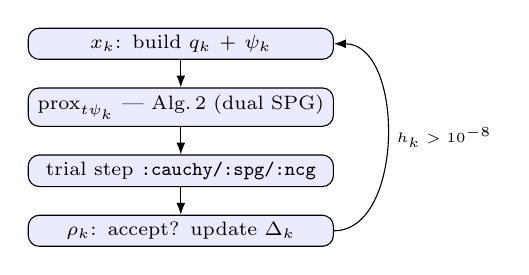
\begin{tikzpicture}[node distance=3.5mm,
       box/.style={draw,rounded corners,fill=blue!8,text width=3.7cm,align=center,inner sep=2.5pt,font=\scriptsize}]
     \node[box](a){$x_k$: build $q_k+\psi_k$};
     \node[box,below=of a](b){$\mathrm{prox}_{t\psi_k}$ --- Alg.\,2 (dual SPG)};
     \node[box,below=of b](c){trial step \texttt{:cauchy/:spg/:ncg}};
     \node[box,below=of c](d){$\rho_k$: accept? update $\Delta_k$};
     \draw[-{Latex[length=1.5mm]}](a)--(b);
     \draw[-{Latex[length=1.5mm]}](b)--(c);
     \draw[-{Latex[length=1.5mm]}](c)--(d);
     \draw[-{Latex[length=1.5mm]}](d.east) .. controls +(0.9,0) and +(0.9,0) .. (a.east)
        node[midway,right,font=\tiny]{$h_k>10^{-8}$};
   \end{tikzpicture}

   \smallskip
   {\footnotesize\raggedright Engineering: type-stable function-barrier \texttt{solve};
   zero-alloc hot kernels; generic \mbox{$T$ (Float32/64/BigFloat)}.\par}
  \end{column}
  \end{columns}
\end{frame}

% ---------------------------------------------------------------- Frame 2
\begin{frame}{Evidence 1 --- the derivatives are correct (finite-difference Taylor test)}
  \small
  \begin{columns}[T]
  \begin{column}{0.56\textwidth}
   Forward differences of the package's nonlinear operator $F$ (\texttt{QuadraticMap}):
   \begin{center}
   \begin{tikzpicture}
   \begin{axis}[width=\textwidth,height=5.6cm,
     xmode=log,ymode=log,
     xlabel={step $h$},ylabel={Taylor remainder},
     legend pos=north west,legend cell align=left,legend style={font=\scriptsize,fill opacity=0.85,text opacity=1},
     grid=both,major grid style={gray!18},minor grid style={gray!8},
     tick label style={font=\scriptsize},label style={font=\scriptsize}]
     \addplot[blue,thick,mark=*,mark size=1pt] table[x index=0,y index=1]{\fdata{jac_taylor.dat}};
     \addlegendentry{$R_0=\lVert F(x{+}hv){-}F(x)\rVert$}
     \addplot[red,thick,mark=square*,mark size=1pt] table[x index=0,y index=2]{\fdata{jac_taylor.dat}};
     \addlegendentry{$R_1=\lVert F(x{+}hv){-}F(x){-}h\,F'(x)v\rVert$}
     \addplot[black!45,dashed,samples=2,domain=1e-8:1]{7*x};
     \addlegendentry{slope 1}
     \addplot[black!45,dotted,samples=2,domain=1e-8:1]{4*x^2};
     \addlegendentry{slope 2}
   \end{axis}
   \end{tikzpicture}
   \end{center}
   {\footnotesize $R_0\!\sim\!\mathcal O(h)$, $R_1\!\sim\!\mathcal O(h^2)$ down to the roundoff floor $\Rightarrow$ $F'(x)$ is exact.}
  \end{column}
  \begin{column}{0.42\textwidth}
   The package ships ROL-style checks; on its (quadratic) testbeds the
   central-difference / identity checks are exact to machine precision:
   \medskip
   {\scriptsize\setlength{\tabcolsep}{3pt}\centering\input{tables/derivchecks.tex}\par}
   \medskip
   {\footnotesize Adjoint consistency and Hessian symmetry are algebraic identities --- verified, not fit.}
  \end{column}
  \end{columns}
\end{frame}

% ---------------------------------------------------------------- Frame 3
\begin{frame}{Evidence 2 --- it finds the true (closed-form) optimum, at every precision}
  \small
  \begin{columns}[T]
  \begin{column}{0.56\textwidth}
   \textbf{Closed-form optima recovered.} LASSO reduction ($A=\{0\}$) matches ROL
   \texttt{test\_01}'s \texttt{getSolution} across all three subsolvers; the
   $\sigma_A=(\cdot)_+$ kink problem hits $x^\star=-\tfrac16\mathbf1$ exactly.
   \medskip
   {\scriptsize\centering\input{tables/closedform.tex}\par}
   \medskip
   {\footnotesize $x^\star_i=\big(\mathrm{clamp}(a_iy_i{+}b_i,-w_i,w_i)-b_i\big)/a_i$ (ROL \texttt{test\_01}).}
  \end{column}
  \begin{column}{0.42\textwidth}
   \textbf{One generic implementation, three precisions.}
   \begin{center}
   \begin{tikzpicture}
   \begin{axis}[width=\textwidth,height=5.2cm,ymode=log,
     xtick={1,2,3},xticklabels={Float32,Float64,BigFloat},
     xmin=0.5,xmax=3.5,ymin=1e-25,ymax=1e-1,
     ylabel={accuracy / tolerance},
     legend pos=north east,legend style={font=\scriptsize},
     tick label style={font=\scriptsize},label style={font=\scriptsize}]
     \addplot[only marks,mark=triangle*,red,mark size=3pt] table[x index=0,y index=2]{\fdata{precision_ladder.dat}};
     \addlegendentry{requested htol}
     \addplot[only marks,mark=*,blue,mark size=2.5pt] table[x index=0,y index=1]{\fdata{precision_ladder.dat}};
     \addlegendentry{achieved $\lVert x-x^\star\rVert$}
   \end{axis}
   \end{tikzpicture}
   \end{center}
   {\footnotesize Same LASSO, \texttt{:spg}, precision-scaled tolerances:
   accuracy meets the requested tol and improves with precision (not a machine-$\varepsilon$ claim).}
  \end{column}
  \end{columns}
\end{frame}

% ---------------------------------------------------------------- Frame 4
\begin{frame}{Evidence 3 --- finite-dimensional E\,+\,CVaR analogue of the paper's risk setting}
  \small
  \begin{columns}[T]
  \begin{column}{0.42\textwidth}
   Same E\,+\,CVaR envelope ($\lambda{=}0.75,\,p{=}0.9$) on a probability-weighted
   $Y$ as the paper --- finite-dimensional (the Burgers/SAA PDE run is \emph{not} reproduced).
   \medskip

   \textbf{Support function is exact} vs.\ an independent water-filling reference,
   both $Y$ metrics, 30 random $y$:
   \medskip
   {\footnotesize\centering\input{tables/cvar_suppA.tex}\par}
   \medskip
   {\footnotesize $J$ convex $\Rightarrow$ $h_k\le10^{-8}$ \emph{certifies} the global optimum.}
  \end{column}
  \begin{column}{0.56\textwidth}
   \textbf{Stationarity $h_k$ vs.\ iteration} --- the improver subsolvers reach the
   paper's target where Cauchy-only stalls:
   \begin{center}
   \begin{tikzpicture}
   \begin{axis}[width=\textwidth,height=5.6cm,ymode=log,
     xlabel={iteration $k$},ylabel={$h_k$},
     legend pos=north east,legend style={font=\scriptsize},
     grid=both,major grid style={gray!18},
     tick label style={font=\scriptsize},label style={font=\scriptsize}]
     \addplot[blue,thick] table[x index=0,y index=1]{\fdata{hk_convergence.dat}};\addlegendentry{\texttt{:cauchy}}
     \addplot[red,thick] table[x index=0,y index=2]{\fdata{hk_convergence.dat}};\addlegendentry{\texttt{:spg}}
     \addplot[green!55!black,thick] table[x index=0,y index=3]{\fdata{hk_convergence.dat}};\addlegendentry{\texttt{:ncg}}
     \addplot[black,densely dashed,samples=2,domain=1:60]{1e-8};\addlegendentry{paper target $10^{-8}$}
   \end{axis}
   \end{tikzpicture}
   \end{center}
  \end{column}
  \end{columns}
\end{frame}

% ---------------------------------------------------------------- Frame 5
\begin{frame}{Evidence 4 --- inexact evaluations honor Conditions 1 \& 2 + provenance}
  \small
  \begin{columns}[T]
  \begin{column}{0.56\textwidth}
   The paper's novel inexactness: admissible model-data error tightens
   automatically as $h_k\!\to\!0$; realized error stays under the bound every iteration.
   \begin{center}
   \begin{tikzpicture}
   \begin{axis}[width=\textwidth,height=5.4cm,ymode=log,
     xlabel={outer iteration $k$},ylabel={error / bound},
     legend pos=south west,legend style={font=\scriptsize},legend cell align=left,
     grid=both,major grid style={gray!18},
     tick label style={font=\scriptsize},label style={font=\scriptsize}]
     \addplot[blue,thick] table[x index=0,y index=1]{\fdata{inexact_records.dat}};
     \addlegendentry{Cond.\,1 bound $\kappa\min(h_k,\Delta_k)$}
     \addplot[blue,only marks,mark=o,mark size=1.3pt] table[x index=0,y index=3]{\fdata{inexact_records.dat}};
     \addlegendentry{realized $\lVert g_k-\nabla f\rVert$}
     \addplot[red,thick] table[x index=0,y index=8]{\fdata{inexact_records.dat}};
     \addlegendentry{Cond.\,2 bound}
     \addplot[red,only marks,mark=square,mark size=1.3pt] table[x index=0,y index=9]{\fdata{inexact_records.dat}};
     \addlegendentry{realized $|\mathrm{ared}-\mathrm{cred}|$}
   \end{axis}
   \end{tikzpicture}
   \end{center}
   {\footnotesize Here realized $=\rho\cdot$bound ($\rho{=}0.5$, by construction); inexact run converges to the exact minimizer.}
  \end{column}
  \begin{column}{0.42\textwidth}
   {\footnotesize\centering\input{tables/inexact.tex}\par}
   \medskip
   \textbf{Provenance.}
   \begin{itemize}\footnotesize\setlength\itemsep{2pt}
    \item ports Trilinos ROL \texttt{TypeP} @\,\texttt{46b83e0}, file-by-file C++ citations
    \item generic over Float32 / Float64 / BigFloat
    \item full suite green: \textit{last verified: 7985 passing (2026-06-18)}

   \end{itemize}
   \smallskip
   {\scriptsize\itshape Scope: a finite-dimensional proof of concept. The match to the
   paper is via theory ($h_k$, Conditions 1\,\&\,2), closed-form / ROL-bridge optima,
   and provenance --- not a live C++ or PDE rerun.}
  \end{column}
  \end{columns}
\end{frame}

\end{document}
